% GNN Calibration Plot - Reliability Diagram
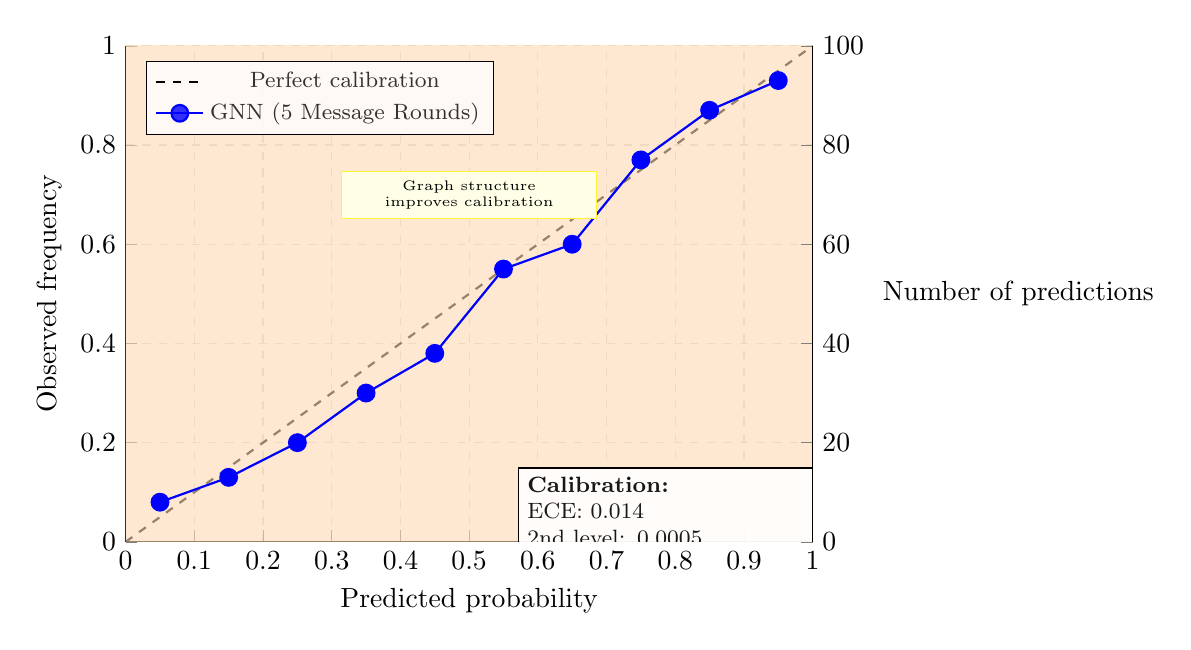
\begin{tikzpicture}
\begin{axis}[
    width=0.85\textwidth,
    height=0.65\textwidth,
    xlabel={Predicted probability},
    ylabel={Observed frequency},
    xmin=0, xmax=1,
    ymin=0, ymax=1,
    grid=major,
    grid style={dashed, gray!30},
    legend pos=north west,
    legend style={font=\footnotesize, fill=white, fill opacity=0.8, draw opacity=1},
    axis y line*=left,
    axis x line*=bottom,
]

% Perfect calibration diagonal
\addplot[dashed, black, thick, domain=0:1] {x};
\addlegendentry{Perfect calibration}

% Histogram bars (number of predictions per bin)
\addplot[ybar interval, fill=orange!30, fill opacity=0.6, draw=none, forget plot] coordinates {
    (0.0, 50) (0.1, 60) (0.2, 65) (0.3, 70) (0.4, 65) (0.5, 60) (0.6, 70) (0.7, 65) (0.8, 75) (0.9, 90) (1.0, 0)
};

% GNN calibration curve
\addplot[color=blue, mark=*, mark size=3pt, thick] coordinates {
    (0.05, 0.08) (0.15, 0.13) (0.25, 0.20) (0.35, 0.30) (0.45, 0.38)
    (0.55, 0.55) (0.65, 0.60) (0.75, 0.77) (0.85, 0.87) (0.95, 0.93)
};
\addlegendentry{GNN (5 Message Rounds)}

% Add calibration metrics annotation box
\node[draw, fill=white, fill opacity=0.9, text width=3.5cm, align=left, font=\footnotesize, anchor=north east] at (axis cs:1.0,0.15) {
    \textbf{Calibration:}\\
    ECE: 0.014\\
    2nd level: 0.0005\\
    90\% Coverage: 87.3\%
};

% Add annotation for graph structure benefit
\node[draw=yellow!80, fill=yellow!10, text width=3cm, align=center, font=\tiny, anchor=south] at (axis cs:0.5,0.65) {
    Graph structure\\
    improves calibration
};

\end{axis}

% Secondary y-axis for number of predictions (right side)
\begin{axis}[
    width=0.85\textwidth,
    height=0.65\textwidth,
    axis y line*=right,
    axis x line=none,
    ylabel={Number of predictions},
    ylabel style={rotate=-90},
    ymin=0, ymax=100,
    xmin=0, xmax=1,
]
\end{axis}

\end{tikzpicture}
